\documentclass[12pt]{article}
 
\usepackage[margin=1in]{geometry} 
\usepackage{amsmath,amsthm,amssymb,bm}
\usepackage{graphicx}
\usepackage{subfig}
\usepackage{array}
 
\newcommand{\N}{\mathbb{N}}
\newcommand{\Z}{\mathbb{Z}}
 
\newenvironment{theorem}[2][Theorem]{\begin{trivlist}
\item[\hskip \labelsep {\bfseries #1}\hskip \labelsep {\bfseries #2.}]}{\end{trivlist}}
\newenvironment{lemma}[2][Lemma]{\begin{trivlist}
\item[\hskip \labelsep {\bfseries #1}\hskip \labelsep {\bfseries #2.}]}{\end{trivlist}}
\newenvironment{exercise}[2][Exercise]{\begin{trivlist}
\item[\hskip \labelsep {\bfseries #1}\hskip \labelsep {\bfseries #2.}]}{\end{trivlist}}
\newenvironment{reflection}[2][Reflection]{\begin{trivlist}
\item[\hskip \labelsep {\bfseries #1}\hskip \labelsep {\bfseries #2.}]}{\end{trivlist}}
\newenvironment{proposition}[2][Proposition]{\begin{trivlist}
\item[\hskip \labelsep {\bfseries #1}\hskip \labelsep {\bfseries #2.}]}{\end{trivlist}}
\newenvironment{corollary}[2][Corollary]{\begin{trivlist}
\item[\hskip \labelsep {\bfseries #1}\hskip \labelsep {\bfseries #2.}]}{\end{trivlist}}

\begin{document}
  
\title{Task 1.2. Supervised Learning: Bayesian Linear Regressor}
\author{Garoe Dorta-Perez\\
CM50246: Machine Learning and AI}
 
\maketitle
 
\section{Introduction}

Simple linear regressors are overconfident in their predictions.
Bayesian linear regressors are an extension of this model used to solve this particular issue.

\section{The problem}

In this model we want to compute a posterior distribution given a set of training samples, as shown in Equation \ref{eq:bayes}. 
Where $\mathbf{w}$ is a one dimensional array with the world state, $\mathbf{X}$ is a matrix with the data points, $\phi$ are the parameters of a linear function of the data.

\begin{equation}
\label{eq:bayes}
Pr(\phi | \mathbf{X}, \mathbf{w} ) = \frac{ Pr(\mathbf{w} | \mathbf{X}, \phi) Pr(\phi)} {Pr(\mathbf{w} | \mathbf{X} )}\,
\end{equation}

The prior in Equation \ref{eq:bayes} is a normal distribution with 0 mean and spherical covariance.
And the likelihood is a multivariate normal distribution, as shown in Equation \ref{eq:normMulti}.
Where  $\sigma^2$ is the covariance, $\mathbf{I}$ is the identity matrix and $\boldsymbol{\theta}= \left\{ \phi, \sigma^2 \right\}$.

\begin{equation}
\label{eq:normMulti}
Pr(\mathbf{w} | \mathbf{X}, \boldsymbol{\theta} ) = Norm_{\mathbf{w}}\left[ \mathbf{X}^T \phi, \sigma^2 \mathbf{I} \right],
\end{equation}

The posterior distribution is: 

\begin{align}
\label{eq:normMulti}
Pr(\phi | \mathbf{X}, \mathbf{w} ) &= Norm_{\phi}\left[ \frac{1}{\sigma^2} \mathbf{A}^{-1} \mathbf{X} \mathbf{w}, \mathbf{A}^{-1} \right],\\
\mathbf{A} &= \frac{1}{\sigma^2} \mathbf{X} \mathbf{X}^T + \frac{1}{\sigma^2_p} \mathbf{I},
\end{align}

\section{Results}


\begin{center}
\begin{tabular}{|c|c|c|c|c|}
\hline
 & $\sigma^2=10$ & $\sigma^2=1$ & $\sigma^2=0.01$ & $\sigma^2=0.001$ \\ \hline
 Font1 & 
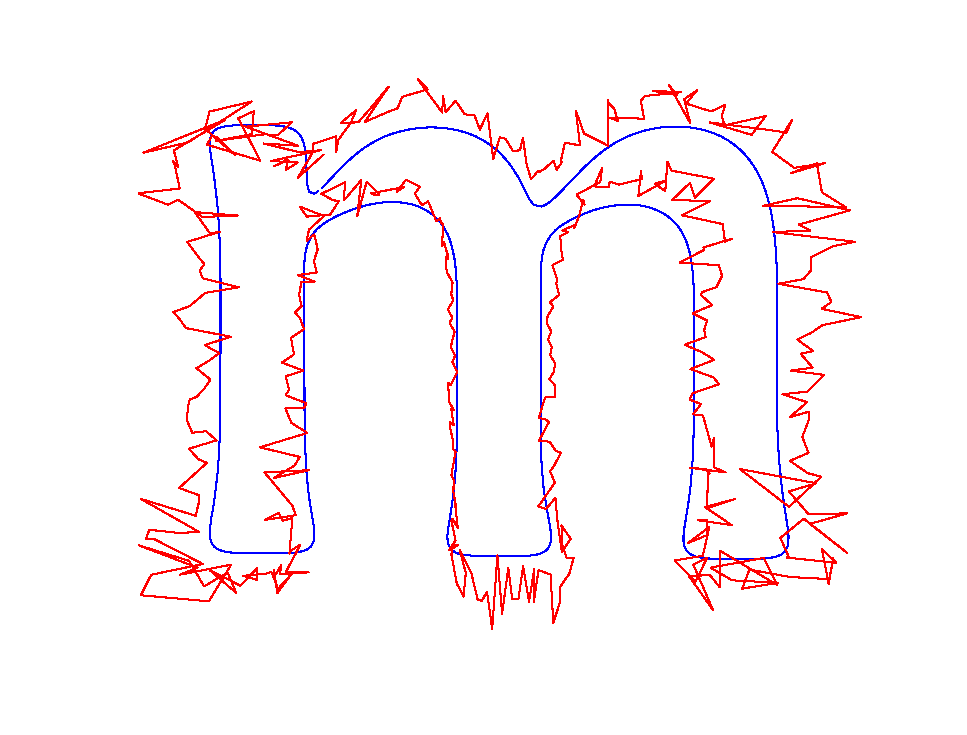
\includegraphics[scale = 0.2]{images/f1var10} &

\includegraphics[scale = 0.2]{images/f1var1} &

\includegraphics[scale = 0.2]{images/f1var0_1} &

\includegraphics[scale = 0.2]{images/f1var0_01} \\ \hline
Font2 & 
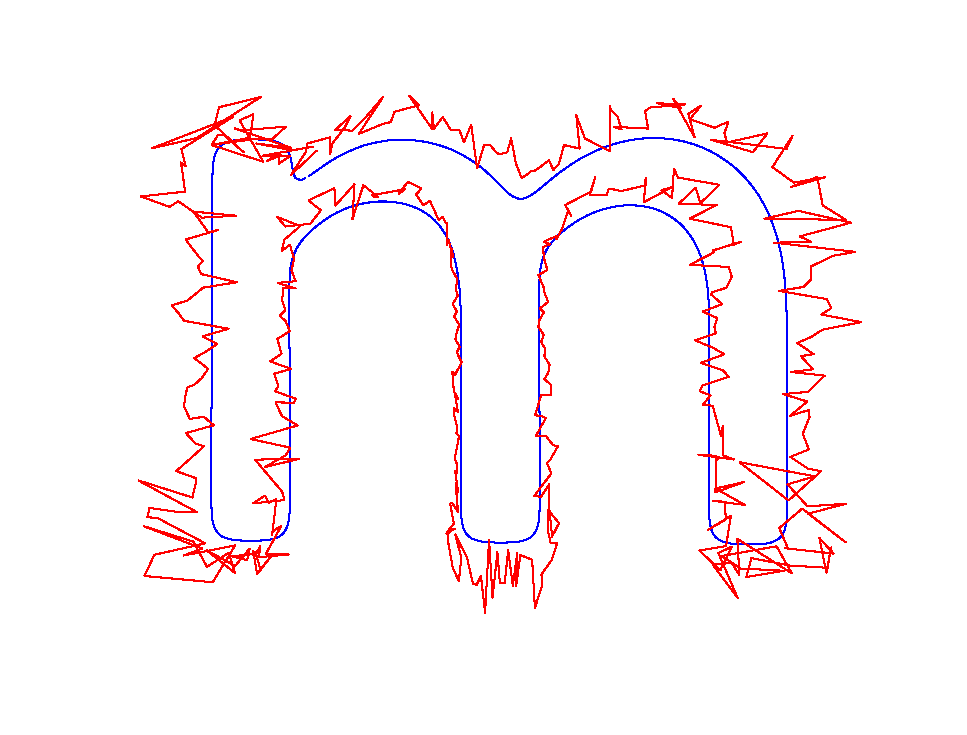
\includegraphics[scale = 0.2]{images/f2var10} &

\includegraphics[scale = 0.2]{images/f2var1} &

\includegraphics[scale = 0.2]{images/f2var0_1} &

\includegraphics[scale = 0.2]{images/f2var0_01} \\ \hline
Font3 & 
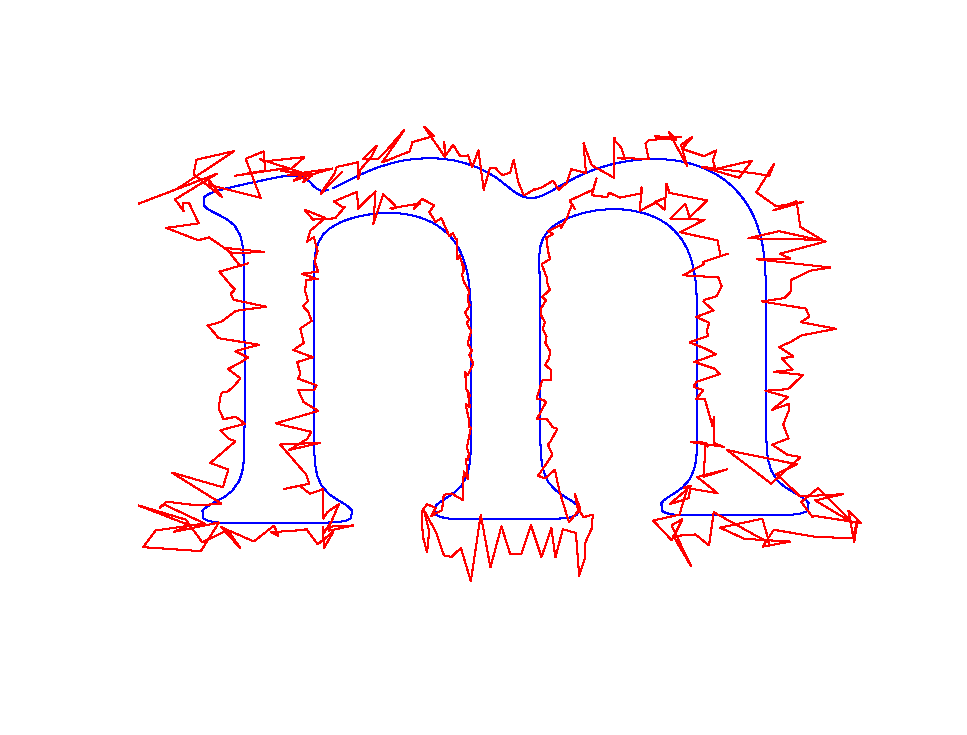
\includegraphics[scale = 0.2]{images/f3var10} &
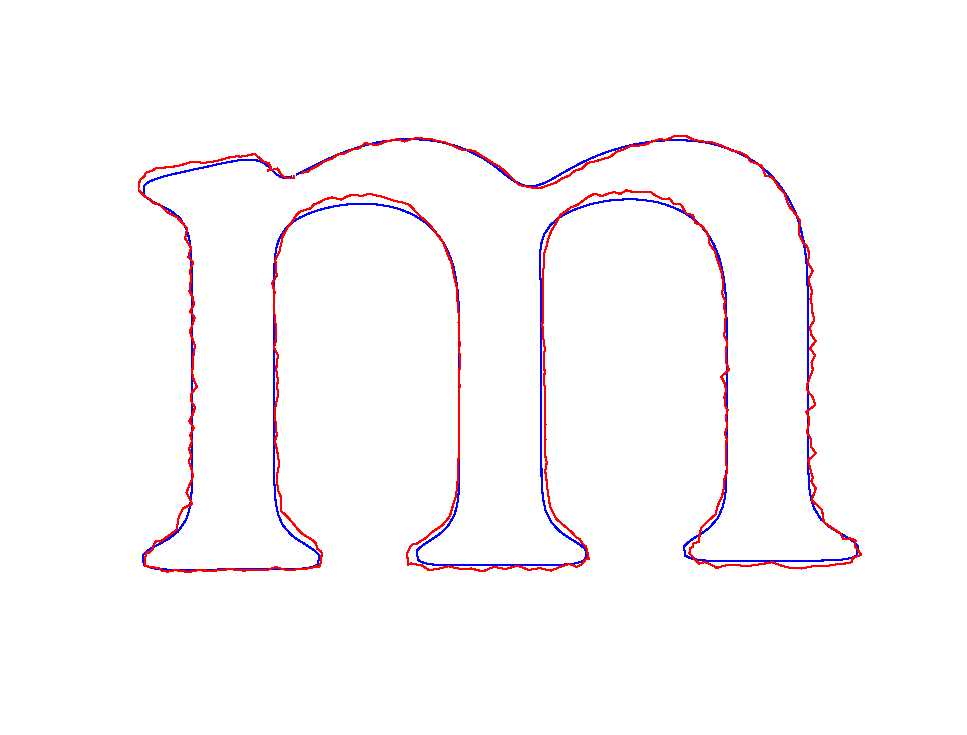
\includegraphics[scale = 0.2]{images/f3var1} &

\includegraphics[scale = 0.2]{images/f3var0_1} &

\includegraphics[scale = 0.2]{images/f3var0_01} \\ \hline
\end{tabular}
\end{center}

\end{document}